\documentclass{article}
\RequirePackage{amssymb}
\RequirePackage{amsmath}
\usepackage{graphicx}
\usepackage[latin1]{inputenc}

\title{Esercizio 2 di riepilogo}
\author{Davide Angelocola}

\begin{document}
\maketitle

\section{Testo del problema}

Sia

$$
P = \begin{pmatrix}
1 & 0 & 0 & 0 & 0 & 0 \cr 
\frac{1}{4} & \frac{1}{2} & \frac{1}{4} & 0 & 0 & 0 \cr 
0 & \frac{1}{5} & \frac{2}{5} & \frac{1}{5} & 0 & \frac{1}{5} \cr 
0 & 0 & 0 & \frac{1}{6} & \frac{1}{3} & \frac{1}{2} \cr 
0 & 0 & 0 & \frac{1}{2} & 0 & \frac{1}{2} \cr 
0 & 0 & 0 & \frac{1}{4} & 0 & \frac{3}{4} \cr 
\end{pmatrix}
$$

matrice di transizione su $S = \{ 1, 2, 3, 4, 5, 6 \}$.

\begin{itemize}
  \item i) Determinare il carattere degli stati
  \item ii) Dimostrare che muovendosi dallo stato 4 con la dinamica descritta da $P$ la probabilit� di raggiungere lo stato 6 in un tempo finito � almeno $\frac{3}{4}$
  \item iii) Calcolare la probabilit� di raggiungere lo stato 1 partendo dallo stato 2 in un tempo finito, $p_{2 1}$ e dare un'interpretazione probabilistica del numero $1 - p_{2 1}$.
  \item iv) Calcolare le eventuali misure invarianti della catena.
  \item v) Determinare la media del tempo di ritorno nello stato 4.
  \item vi) Per la catena con matrice di transizione P e densit� iniziale uniforme su $\{4,5,6\}$, calcolare la probabilit� degli eventi $A = \{X_2=4\}$, $B = \{X_2 = 4, X_3 = 5\}$ e $C = \{X_100 =4, X_101 = 2\}$. In che modo si potrebbe procedere per calcolare in modo approssimato
\end{itemize}

\section{i) Carattere degli stati}

Disegnamo il grafo delle transizioni:

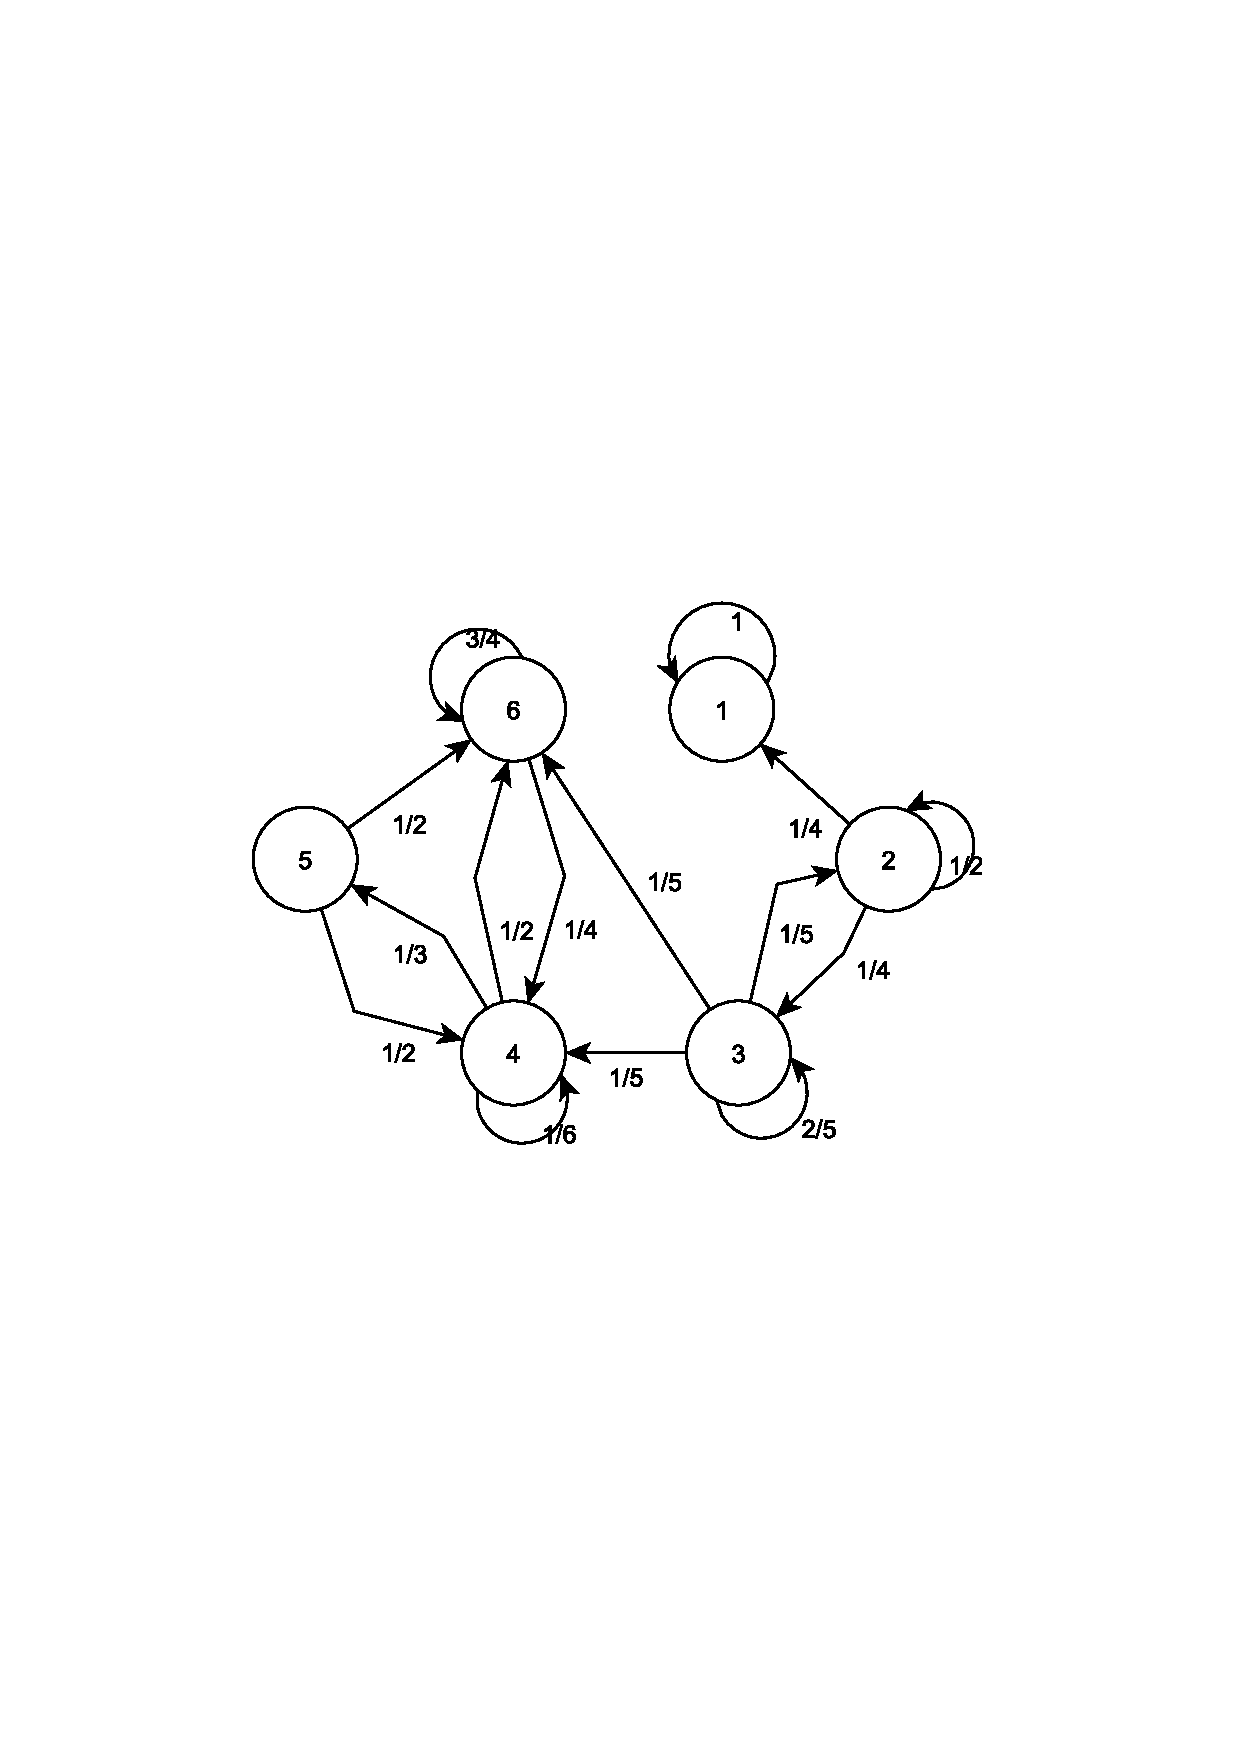
\includegraphics[scale=0.5]{cp_ex2_fig1.pdf}

\begin{enumerate}
  \item � uno stato assorbente
  \item � uno stato transiente perch� comunica con 1 ma non � ricambiato
  \item � anch'esso transiente perch� comunica sia con 4 sia con 6 ma non � ricambiato
  \item forma, insieme agli stati 5 e 6, una classe irriducibile \footnote{cosa sono gli stati persistenti positivi?}
  \item forma, insieme agli stati 4 e 6, una classe irriducibile
  \item forma, insieme agli stati 4 e 5, una classe irriducibile
\end{enumerate}

\section{ii)}

Considerando la classe irriducibile trasformata in modo tale che lo stato 6 sia assorbente:

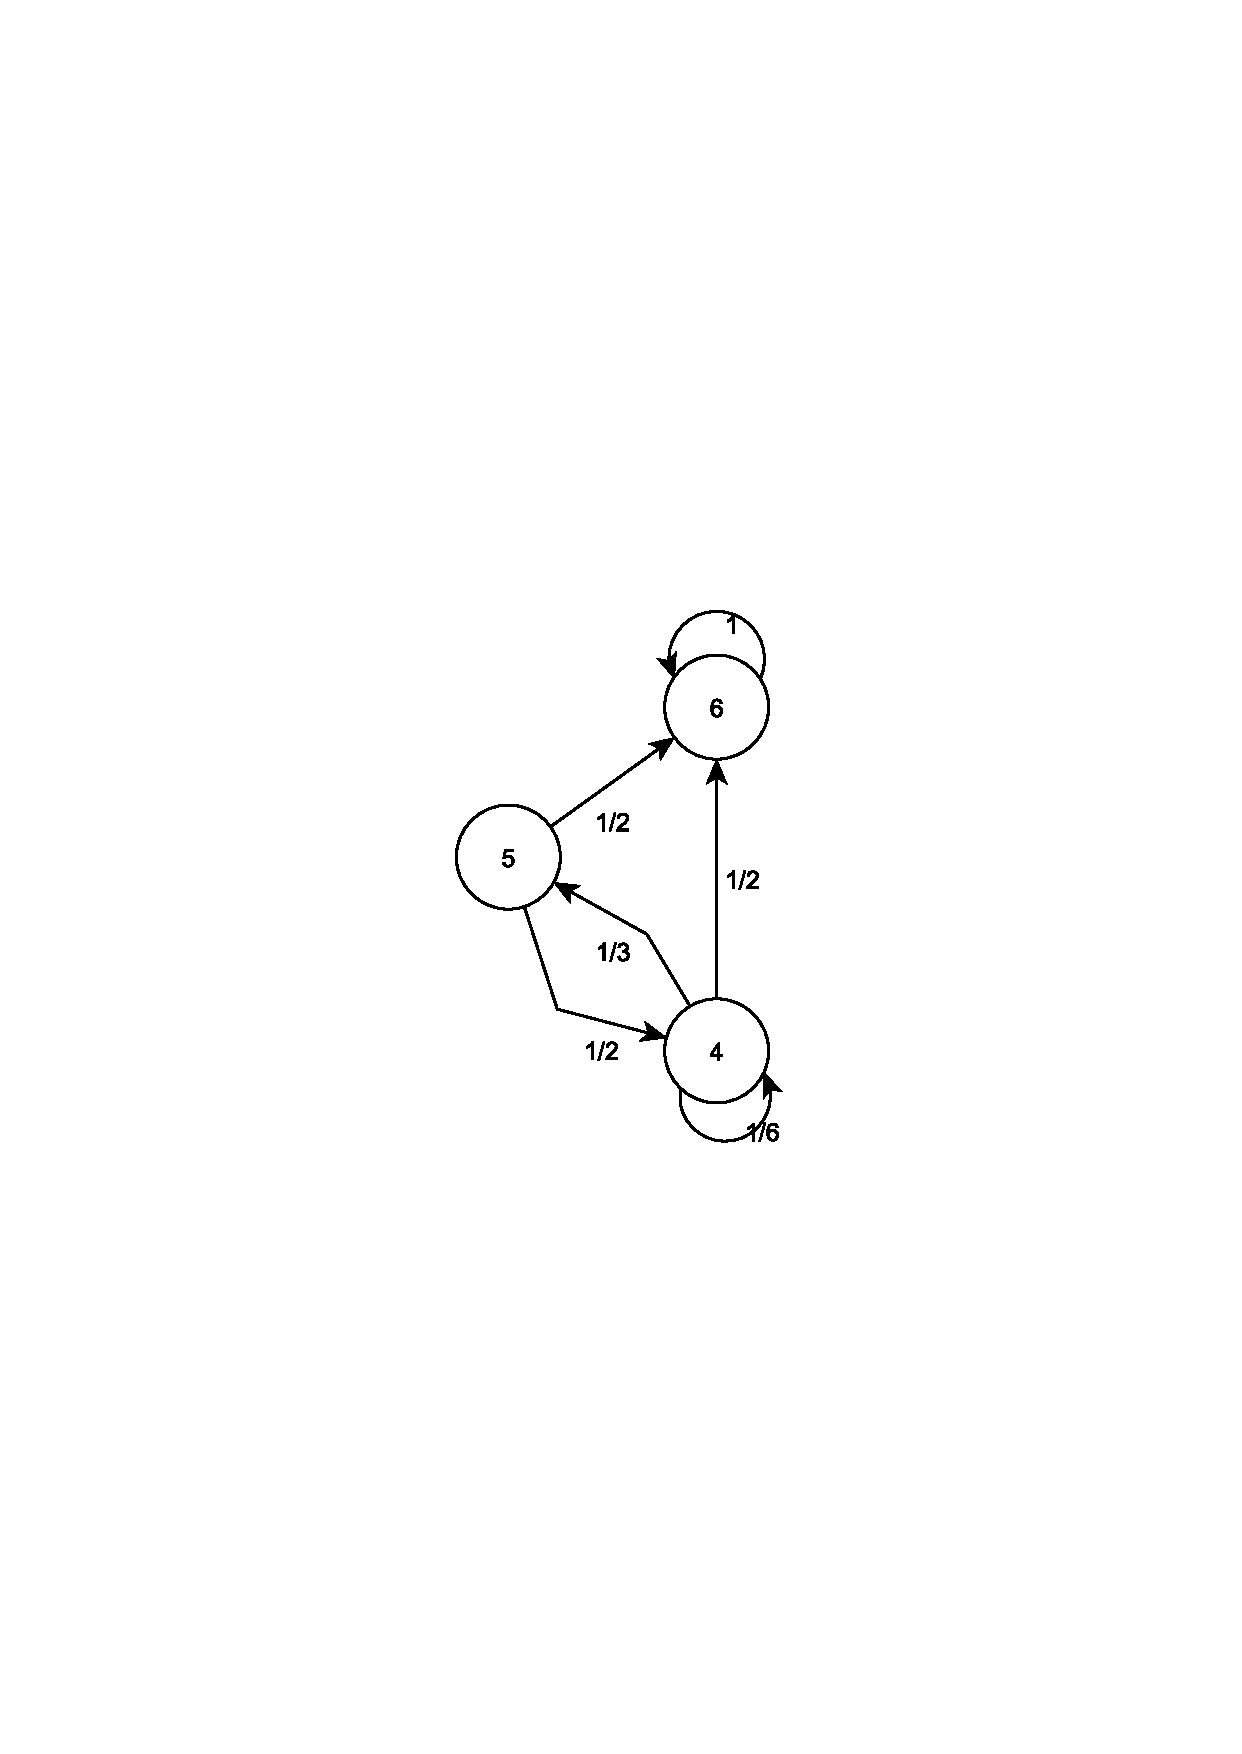
\includegraphics[scale=0.5]{cp_ex2_fig2.pdf}

Possiamo quindi andare da 4 a 6 in 1 passo (minorazione):

$$
\rho_{46} \ge \rho_{46}^{(1)} = p_{46} = \frac{1}{2}
$$

in due passi si possono prendere diverse percorsi in 2 passi:

$$
\rho_{46} \ge \rho_{46}^{(1)} + \rho_{46}^{(2)} = p_{46} + (p_{45} + p_{56}) + (p_{44} + p_{46}) = \frac{3}{4}
$$

\section{iii)}

Essendo lo stato 1 assorbente per calcolare la probabilit� di raggiungerlo in tempo finito a partire da $2$ occorre calcolare $\lambda_2^{\{1\}}$ usando:
 
\begin{equation} 
x_i = \sum_{j \in S \backslash T}{p_{i j}} + \sum_{j \in T}{p_{i j}x_j}, \forall i \in T
 \label{eq:1}
\end{equation}

Risolvendo il sistema:

$$x_2=\frac{1}{4} + \frac{1}{2}x_2 + \frac{1}{4}x_3$$
$$x_3=\frac{1}{5}x_2 + \frac{2}{}x_3$$

si ottiene:

$$x_2 = \frac{3}{5}$$ 
$$x_3 = \frac{1}{5}$$

La quantit� $1 - \rho_{21}$ � la probabilit� di non essere assorbiti in $1$ in un tempo finito. Per la natura di questa catena ci� equivale ad essere assorbiti nella classe irriducibile ${4, 5, 6}$. Poich� gli stati transienti sono in numero finito intuitivamente si deve "cadere" o nella classe ${1}$ o nella classe ${4, 5, 6}$. 

\section{iv}\label{sec:iv}
 Poich� 1 � stato assorbente la prima misura invariante $v^{(1)}$ � quella che assegna 1 allo stato assorbente 1 e 0 agli stati transienti (2 e 3):

$$
v^{(1)} = (1\ 0\ 0\ 0\ 0\ 0\ 0)
$$

L'altra classe chiusa � quella relativa agli stati 4 5 e 6. Risolvendo il sistema sulle equazioni si ottiene il vettore $v^{(2)}$:

$$v = v \times P = (x_1\ x_2\ x_3\ x_4\ x_5\ x_6) P $$

%% TODO: finire di scrivere il sistema 

\section{v}\label{sec:v}
La sottocatena $S_1 = {4, 5, 6}$ in quanto � finita e irriducibile (quindi persistente e positiva). La sua misura invariante, calcolata in \ref{sec:iv}, �  
$v = (\frac{1}{4} \frac{1}{12} \frac{2}{3})$. Il tempo medio di ritorno nello stato 4 �:

$$
E[t_4] = \frac{1}{v_4} = \frac{1}{\frac{1}{4}} = 4 
$$

\section{vi}
Considerando solo la classe chiusa formata dalla sottocatena $S_1 = {4, 5, 6}$. Occorre calcolare $P^2$:

$$
P(A) = \frac{1}{3}(p_{44}+p_{45}+p_{46})
$$

di $P^2$. Usando la markovienet� � facile calcolare $P(B)$:

$$P(B) = P(A)  p_{45}$$

Poich� 4 non comunica con 2 si ha che:

$$
P(C) = 0
$$

Infine per il calcolo di $P(D)$ si fanno le seguenti deduzioni: la catena � irriducibile e finita, poich� almeno uno stato ha $p_{ii} > 0$ si conclude che essa � aperiodica (t=1). Per una catena irriducibile il fatto che sia finita e aperiodica implica che sia ergotica, e quindi che ammette una unica misura invariante che coincide con quella "a regime". Essendo 50 un numero abbastanza grande possiamo applicare il limite, ottenendo quindi $\frac{1}{12}$ ovvero $v_4$ calcolato al punto \ref{sec:v}.

\end{document}
